\title {BIP ESMoL Integration Design Document}
\author {Mohamad Jaber, Graham Hemingway, Joseph Porter}
\maketitle

\section{Goals}

Long-Term Goal: Extend ESMoL to import BIP design models and generate BIP verification models with platform effects included.

Short-Term Goals:

\begin{enumerate}
\item Get an example working end-to-end with the socket simulation.
\item Do another example including Simulink functions invoked by BIP.
\item Create a full BIP model from an example, including platform effects.
\item Extend the virtual machine and scheduler for sporadic, event-driven tasks.
\item Do an end-to-end example including Simulink, BIP generation, and synthesis to the virtual machine.
\end{enumerate}

\subsection{ESMoL Overview}

\begin{figure}[htb]
	\centering
		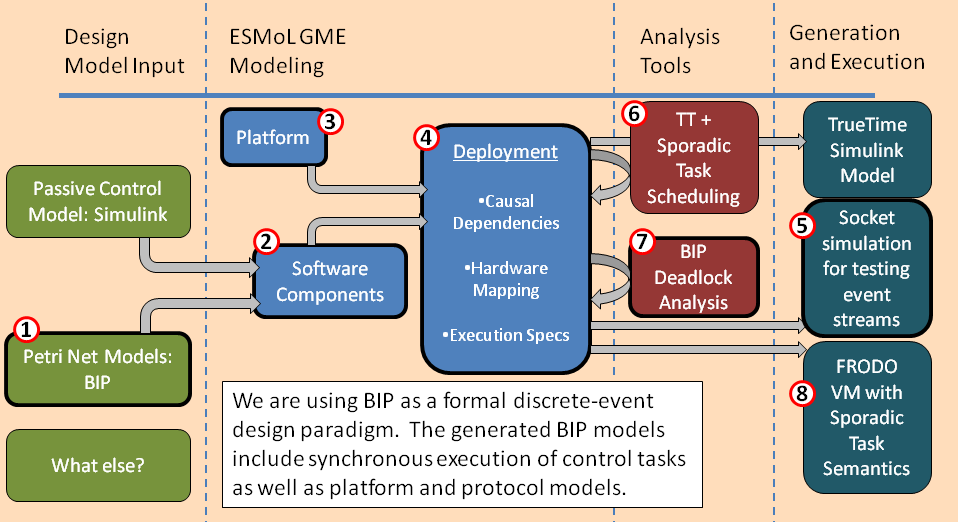
\includegraphics[width=1.00\textwidth]{figures/tool_diagram.png}
	\caption{Flow of models in the design process.}
	\label{fig:tool_diagram}
\end{figure}

ESMoL supports a model-based design flow for embedded systems.  The process is shown in Fig. \ref{fig:tool_diagram}.

\begin{enumerate}
\item Import design models from other languages (here we are interested in BIP). 
\item Blocks in the imported language are used to define components in the design language.
\item User specifies the platform topology and its parameters.
\item User specifies the component-to-hardware deployment mapping.
\item We generate socket implementations in order to test event-driven applications.
\item The scheduling tool uses specified timing and execution frequency bounds to determine schedulability and calculate start times for time-triggered tasks.
\item The BIP model is re-generated with the platform models included (for analysis).
\item We generate an implementation in C to run on the virtual machine.
\end{enumerate}

\subsection{Things to Do}

\subsubsection{Goal 1: Socket Simulation}
\begin{enumerate}
\item Create a useful BIP example involving multiple event-triggered inputs.
\item Create templates for socket simulation output.
\item Integrate socket output into the stage2 generator.
\end{enumerate}

Questions / issues:

\begin{enumerate}
\item How do we specify the timing characteristics of the sporadic input events in ESMoL?
\item How do we calculate schedulability for the specified events?
\end{enumerate}

\subsubsection{Goal 2: Simulink invoked by BIP}
\begin{enumerate}
\item Extend the example to use Simulink-specified components (or make a new example).
\item Create a BIP template for a Simulink dataflow model, including preemption.
\item Extend the scheduler model to include constraints for sporadic tasks.
\end{enumerate}

\subsubsection{Goal 3: Generating BIP (including Platform)}
\begin{enumerate}
\item Create BIP templates for execution of the virtual machine and communications.
\item Extend Stage2 with BIP generation.
\end{enumerate}

\subsection{Things Done}

\begin{enumerate}
\item 10/14/2009 Created this spec document!!!
\end{enumerate}